\chapter{基于模型量化和查找表的矩阵向量乘软件优化}

\section{量化基本说明}
基于在第二章介绍的GEMV的通用两种方法,直接使用float32数据格式进行GEMV的计算的性能非常差,原因是UPMEM硬件不支持浮点数的算术运算而使用软件模拟,其性能大约是int32数据类型格式的算术吞吐的十分之一\cite{BenchmarkingMutlu},因此需要将权重矩阵和激活向量量化到8bit进行计算。在上一小节提到,浮点量化格式往往优于定点数量化\cite{ZeroQuantFP};同时测试表明UPMEM的读写速度相较于其计算核心更快,计算访存比仅有1:4\cite{BenchmarkingMutlu},因此非常适合用访存换计算。我们直接使用基于FP8数据格式的查找表算法,会比直接使用int8的矩阵向量乘法内核的“性价比”更高(模型精度/算子性能)。为提高量化精度我们可以使用机器学习的方式以少量的校准数据集调整量化后参数,针对反向传播中LUT不可导的问题,可以使用直通估计器(Straight-Through Estimator,STE)解决\cite{NonuniformQuant}。STE简单来说就是跳过LUT自身的梯度下降,将误差直通传递到上一层,如通过调整上一层的矩阵权重来实现误差最小化,这是一种非均匀量化的手段。

本章所讨论的权重矩阵和激活向量的维度如果没有说明都和Llama2-7B保持一致为4096,权重矩阵的维度为$4096\times 4096$,分到32个头后,单个DPU负责一个头的自注意力计算(算子融合),矩阵的维度为$4096\times 128$,本章所有讨论的优化都是建立在单个DPU的推理优化。因此单个DPU的GEMV内核的正常输入为4096维度FP8数据格式的激活向量,4096维度FP8数据格式的权重方阵,最终计算得到的结果也应该是4096维度的结果向量。

UPMEM的MRAM访问通过DMA引擎速度较慢,并且需要大批量数据传输,应该尽量减少MRAM的访问。UPMEM访问WRAM的速度较快,当流水线充满时,且访问带宽不受访问模式影响(顺序、随机),且任何8byte以下的数据访问都只会消耗一个时钟周期。这里为后续算法做时间复杂度分析,建模WRAM的一次读或写消耗为$read$。

\section{基于查找表分块的矩阵向量乘算法}
\subsection{矩阵向量乘查找表基础}
查找表(LUT)是非常典型的存储换计算的技巧,常常被用在某些边端设备或者计算能力有限的硬件上以支持复杂计算。由于UPMEM硬件本身较弱的计算能力,以及较低的计算访存比,非常适合使用访存换计算的方法。一般意义上的查找表就是对于函数$f(x_1,x_2,\cdots,x_n)=y$,在一定的定义域范围和精度内穷举所有自变量的组合,并提前计算得到每种组合对应的函数值,制作成一张映射表,此后的函数计算无需计算而只需查表即可。由于计算机只能离散有限地表示数值,每种特定位宽的数是天然可穷举的,例如对于$n bit$的数作为自变量,其本身有$2^n$种不同的数值,两个$n bit$的数作为自变量,则有$2^{2n}$个不同的组合。

\begin{figure}[!htbp]
	\centering
    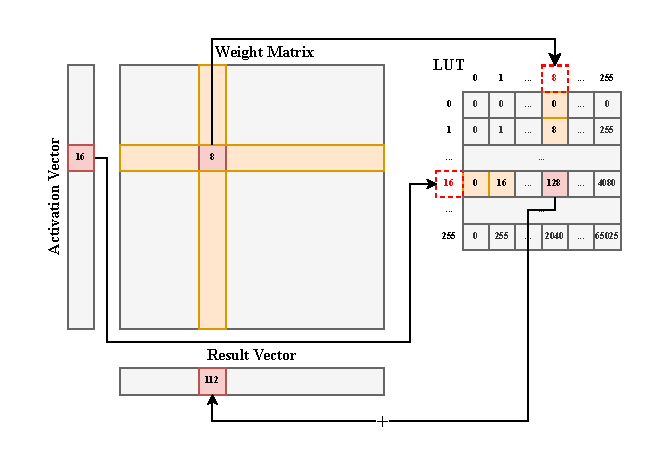
\includegraphics[width=0.9\textwidth]{figures/LUT.pdf}
	\caption{使用查找表卸载GEMV中的乘法示意图}
    \label{LUT}
\end{figure}

这里举例GEMV的8bit乘法查找表的设计,如图\ref{LUT}所示,其中有一张数据类型为uint8的乘法查找表(为了直观采用uint8数据格式)。由于两个操作数都为8bit,因此输入一共有$256\times 256=2^{16}$种组合,因此可以提前构建一个256行256列二维数组存储查找表,第一个操作数的数值代表行索引,第二个操作数的数值代表列索引,行索引和列索引交叉索引到的元素值为两个操作数的乘积。例如在进行GEMV运算时,要计算激活向量中某个值为16的元素和权重矩阵中某个值为8的元素的乘积,现只需要访问提前构建好的二维数组(查找表)的第16行第8列的元素即可,得到答案为128,再加到结果向量的对应位置上。当然这里加法计算同样可以通过构建一张8bit的加法查找表消除。这样,8位宽下任意数据格式的任意二元算术运算都可以按照上述的查表方式将计算转换为访存。同时上述访存过程仅仅涉及最简单的数组索引计算,几乎能够得到所有硬件的支持,从而降低了对硬件算术能力的要求。

上述乘法查找表的构建存在冗余,因为乘法满足交换律,因此上述$256\times 256$的矩阵只需要保存上三角或下三角即可。甚至能够进一步将8bit的乘法拆成4bit的乘法的加法,但这两种做法无疑都会增加计算复杂度,对于在UPMEM上需要频繁访问的查找表而言是不合适的。同时查找表能够按照行划分成为子表,例如上述uint8的乘法查找表,当能够确定某个操作数的变化范围在[0,64)时,只需要上述查找表的前64行即可满足计算,即每一行和多行的组合都是属于8bit乘法查找表的子查找表,当空间受限时,可以按需载入子查找表。在此我们特别约定,1)查找表的大小和构建方式都如上述所描述,n bit的二元运算查找表表项为$2^{2n}$;2)二元运算查找表通过两个索引(分别是行列索引)确定查找值,约定这里的索引在后文称作索引值(row/col index),查表得到的值为元素值(element);3)后文如果没有特别说明,子查找表指的是原查找表二维数组的不同行的组合,即确定行索引值的范围的子表。

\subsection{分块载入查找表卸载乘法}
直接使用8bit乘法查找表的方法在UPMEM中卸载GEMV计算存在诸多问题,首当其冲的就是WRAM的空间限制:由于查找表在执行GEMV运算时需要频繁访问,因此必须要将其载入WRAM这种高速内存中才会有较好的性能。然而8bit的查找表光是表项就有$256x256=2^{16}=64K$项,如果按照表中每个元素刚好占用1字节,则查找表需要占用空间64KB,而WRAM的容量只有64KB,除了用户数据之外至少需要为各个线程的堆栈留存一部分空间,因此无法将整个查找表载入WRAM。

解决办法就是分块载入查找表,每次只执行数据范围落在当前载入的子查找表覆盖的范围内的计算。但是此时需要注意的一点就是在于数据的重用性:权重矩阵无法一次性全部载入WRAM,从MRAM载入WRAM的带宽远低于WRAM与核心交互的带宽,分多次载入子查找表后需要避免因为计算不完整而重复载入矩阵。基于上述考虑,我们设计了基于分块载入查找表卸载GEMV中的乘法的算法,具体如图\ref{LUTBlock}所示,激活向量和结果向量完整载入WRAM中,将查找表拆分成16个子查找表,行索引范围被划分为在$[0-15),[16-31),\cdots,[240,256)$16个区间。该算法需要进行子查找表次数个迭代,每次迭代流程大致为:将子查找表载入WRAM中,遍历激活向量,对于每个元素判断其值是否在当前子查找表的索引值区间内,对于满足要求的元素,将该元素所对应的矩阵的行向量从MRAM载入WRAM,执行查表乘法计算并加到结果向量上;对于不满足要求的元素直接跳过,等待下一次迭代再进行判断。如此一来完全没有将数据重复地从MRAM搬移到WRAM中,无论是查找表还是权重矩阵,都只从MRAM中搬移到WRAM中一次,实现了非常的WRAM数据局部性。

\begin{figure}[!htbp]
	\centering
    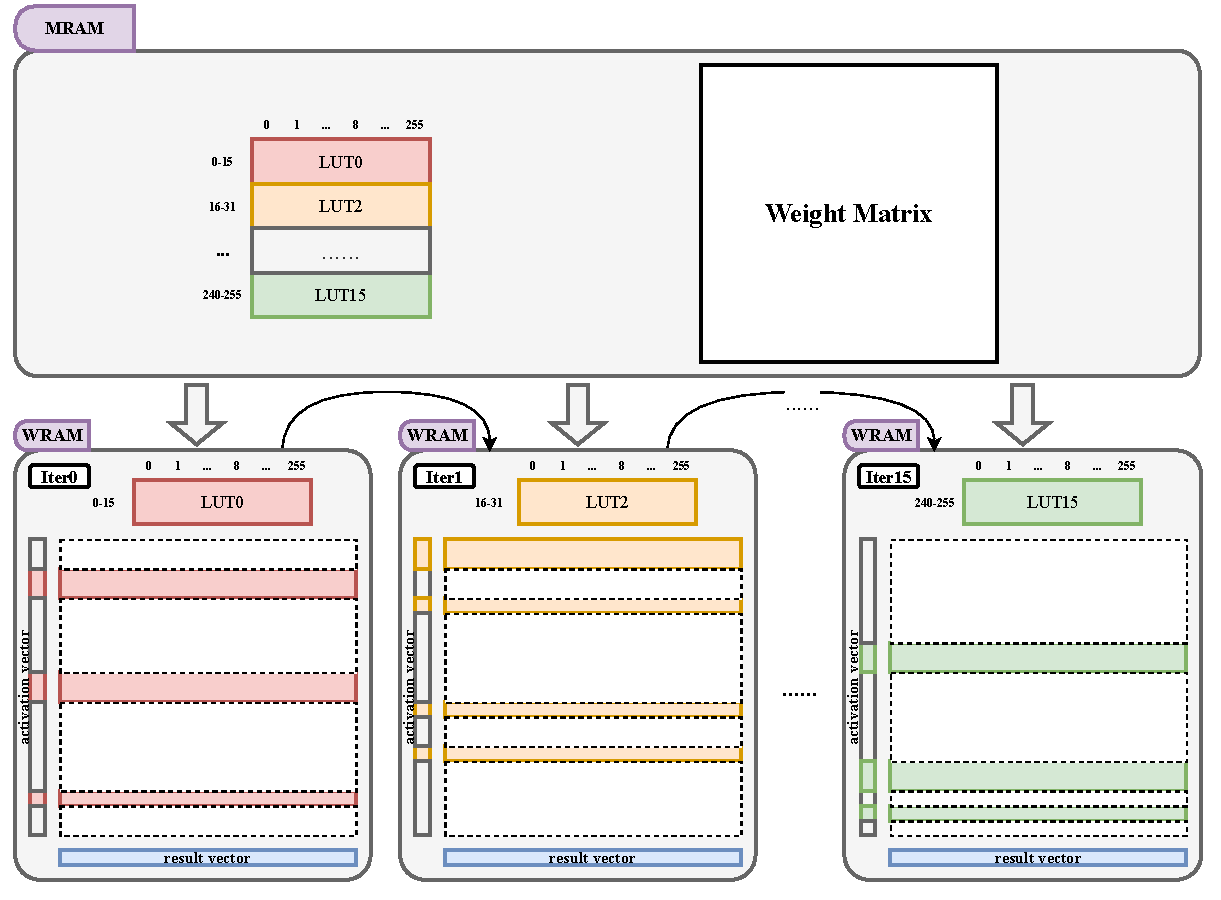
\includegraphics[width=0.9\textwidth]{figures/LUTBlock.pdf}
	\caption{分块载入查找表卸载GEMV的算子乘法示意图,图上面表示MRAM中存放的数据,图下面表示WRAM和迭代计算}
    \label{LUTBlock}
\end{figure}

\subsection{基于数制映射表卸载加法}
想要完整卸载GEMV算子的所有计算仅仅使用上述分块查找表卸载乘法远远不够,上述方法虽然使用分块载入的方式解决空间上的限制,但是在计算加法时如果想要使用类似的思路,由于使用的数制是FP8,硬件加法无法支持,同时由于累加的操作特性,FP8加法的所在查找表区间是动态变化的,无法事先静态地确定并载入子查找表,直接从MRAM中读取性能就会非常差。一种方式是直接使用软件模拟:FP8常用的有两种格式\cite{FP8},如表\ref{FP8Format}所示,我们选用E4M3格式的FP8进行推理,因其相较于E5M2具有更高的精度(E5M2相较于E4M3拥有更高的动态范围更适合训练)。其数据格式并不完全符合IEEE754,取消了无穷的表示缩减了NaN的表示范围以容纳更多规格化数,其他部分均符合IEEE754的标准。
    
\begin{table}[!htbp]
    \caption{FP8常用两种格式二进制细节}
    \label{FP8Format}
    \begin{tabular}{lll}
        \toprule
        & E4M3 & E5M2 \\ 
        \midrule
        Exponent bias & 7 & 15 \\
        Infinities & N/A & S.11111.00\textsubscript{2} \\
        NaN & S.11111.11\textsubscript{2} & S.11111.\{01, 10, 11\}\textsubscript{2} \\
        Zeros & S.0000.00\textsubscript{2} & S.00000.00\textsubscript{2} \\
        Max normal & S.1111.10\textsubscript{2} = 1.75 * 2\textsuperscript{8} = 448 & S.11110.11\textsubscript{2} = 1.75 * 2\textsuperscript{15} = 57,344 \\
        Min normal & S.0001.00\textsubscript{2} = 2\textsuperscript{-6} & S.000001.00\textsubscript{2} = 2\textsuperscript{-14} \\
        Max subnormal & S.0000.11\textsubscript{2} = 0.875 * 2\textsuperscript{-6} & S.000000.11\textsubscript{2} = 0.75 * 2\textsuperscript{-14} \\
        Min subnormal & S.0000.01\textsubscript{2} = 2\textsuperscript{-9} & S.000000.01\textsubscript{2} = 2\textsuperscript{-16} \\ 
        \bottomrule
    \end{tabular}
\end{table}

如果直接使用软件模拟,计算两个浮点数的流程的大致为:对阶、尾数求和、规格化、舍入、溢出处理,虽然不用处理无穷等特殊情况,但是上述几个步骤中涉及到大量的移位操作和逻辑操作,由于UPMEM的一个周期至多只能执行一条指令\cite{UPMEMHotChips},因此这些位运算和逻辑运算指令开销不能忽视,而且由于规格和非规格数的区别存在大量的条件判断和跳转语句,同样非常影响性能。我们注意到,可以将E4M3格式的FP8展开成int32,使用int32进行加法计算和中间结果的保存(硬件不支持int32乘法但是支持加法),在得到最终的结果向量后再转回FP
8数制以便后续的传输。具体的展开形式可以很简单,E4M3的符号位不变置于int32的符号位,同时根据指数位置判断该数是否为规格化数,若是规格化数,则需要将尾数的低三位前面添1形成4位尾数;若不是规格化数,则正常取尾数。然后假设指数部分的值为e,将尾数左移$max(e-1,0)$位即可。如图\ref{LUTBS}所示,FP8数0 0010 110转为int32为0...11100,FP8数0 0000 110转为int32为0...110,二者相加得0...100010,这个时候反转回FP8应该首先判断是否为规格数,显然该数为规格化数,需要将int32数右移直至前导第一个1到最低第4位上(计算舍入)即可。

但其实同样可以使用一张数制映射表代替上述复杂的逻辑操作,如图\ref{LUTBS}中的FP8\_TO\_INT32\_LUT,是一个表项为256的一元映射查找表,提前将FP8展开存储在该张映射表中,在计算时展开操作就可以换为查表操作。更进一步,原本的乘法查找表元素为单字节FP8,现在将其替换为其对int32的映射项,变为四字节。这样查询出来的乘积就是int32的展开格式,直接加到同样每个元素扩展为32位的结果向量中。最后,基于查找表FP8\_TO\_INT32\_LUT再通过二分查找将结果向量中的每个元素还原成FP8以便后续的传输。

\begin{figure}[!htbp]
	\centering
    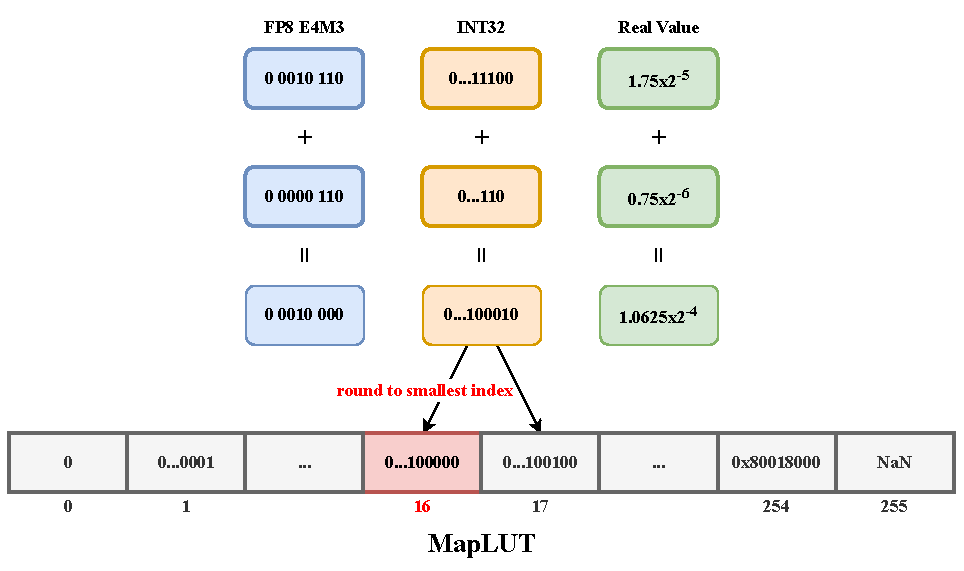
\includegraphics[width=0.9\textwidth]{figures/BinarySearch.pdf}
	\caption{分块载入查找表卸载GEMV的算子乘法示意图,图上面表示MRAM中存放的数据,图下面表示WRAM和迭代计算}
    \label{LUTBS}
\end{figure}

在查找的过程中,可能会遇到舍入问题,即计算出来的元素值无法精准匹配查找表中的元素,其原因是使用int32进行加法运算时保留了相当的精度没有舍入,这个时候会出现待查找的值处于查找表两个相邻元素值之间,如图\ref{LUTBS}所示,为了简化计算加速查找我们直接选择索引值较小的那个数作为查找结果:一方面转为int32进行中间结果的加法运算相对于直接使用FP8计算保留了相当大精度,这里只是将最终结果进行转换因此精度损失整体来讲不大;另一方面精度损失仍然可以通过离线的基于机器学习的量化工作优化消除。这种舍入方式我们这里称之为向最小索引值舍入(Round to Smallest Index),这种舍入其实本质和向零舍入(Round toward Zero)是同一种舍入规则。

\subsection{算法小结}
至此,可以完全卸载GEMV算子的全部运算到UPMEM上,我们在这里对上述方法进行总结,给出算法如\ref{LUT_Block}所示,假设M和N都为4096,那么激活向量大小为4KB,8bit和32bit的结果向量的大小分别为4KB和16KB,将查找表分成16份,每个子查找表的大小为16KB,载入的矩阵一行的大小为4KB,FP8到int32的映射表大小为1KB,总共占用WRAM空间45KB,剩余19KB给各个线程分配堆栈空间完全足够用。在这种设计下,权重矩阵的所有行总共只需要从MRAM中载入WRAM中一次,LUT的每个子表同样也只载入一次,FP8和int32的相互映射也是直接在WRAM中完成,充分提高了数据的重用性。

\begin{algorithm}[!ht]
    \caption{基于查找表分块的矩阵向量乘算法-LUTBlock}
    \label{LUT_Block}
    \begin{algorithmic}[1]
        \Require $Vector[M], Matrix[M][N], LUT[256][256], FP8\_to\_INT32[256]$; % input
        \Ensure $Result\_8[N]$; % output

        \State $\textbf{define}\; SubLUT[16][256]$
        \State $\textbf{define}\; MatRow[N]$

        \For{$i \gets 0$ \textbf{to} $15$}
            \State $\textbf{mram\_read}(SubLUT, LUT[16i \cdots 16i + 15])$
            \Comment{\textcolor{blue}{parallel in 16 for each tasklet}}
            \For{$j \gets 0$ \textbf{to} $M - 1$}
                \If{$Vector[j] \;\textbf{not in}\; [16i, 16i+15]$}
                    \State \textbf{continue}
                \EndIf
                \State $\textbf{mram\_read}(MatRow, Matrix[j])$
                \Comment{\textcolor{blue}{parallel in N for each tasklet}}
                
                \For{$k \gets 0$ \textbf{to} $N-1$}
                \Comment{\textcolor{blue}{parallel in N for each tasklet}}
                    \State $Result[k] \gets Result[k] + SubLUT[Vector[j] \& \text{0xF}][MatRow[k]]$
                \EndFor
            \EndFor
        \EndFor

        % 调用二分查找函数
        \State $\textbf{define}\; Result\_32[N]$
        \State $Result\_8 \gets \textbf{BinarySearch}(Result\_32, FP8\_to\_INT32)$
        \Comment{\textcolor{blue}{parallel in N for each tasklet}}
        \State \Return $Result\_8$
    \end{algorithmic}
\end{algorithm}

\section{针对不同尺寸矩阵的矩阵向量乘优化}
在上一小节主要针对MRAM的读写做了优化,提高了WRAM的数据局部性,这一小节主要针对WRAM做优化,提高寄存器的数据重用。

我们知道在Llama2-7B的MHSA中,会将一个完整的4096长度的词向量通过线形层成映射到32个子空间,对应到32个头(会将$4096\times 1$的向量映射成32个$128\times 1$的向量),本质上属于降维操作,(单个头)线形层是一个$4096\times 128$的窄矩阵;在最终计算得到attention向量后,又会通过一个线性层将$128\times 1$的向量重新映射为$4096\times 1$并最终合并各个头的结果,属于升维操作,此时线形层是一个$128\times 4096$的宽矩阵。一般意义上,对于一个$M\times N$的矩阵,当$M\gg N$时,认为这个矩阵是所谓的窄矩阵;当$M\ll N$时,认为这个矩阵是所谓的窄矩阵,但这里我们认为$4096\times 128$或$4096\times 256$就属于窄矩阵,$128\times 4096$或$256\times 4096$就属于宽矩阵(并且在后文中使用128维度作为示例)。这两种形状的矩阵在LLM的推理过程中十分常见(MLP部分的矩阵可以随意切),可以针对这两种特殊的矩阵进行优化。

\subsection{窄矩阵行重排}
对于窄矩阵($4096\times 128$),其特点在于行数相较于列数非常多,频繁地读写结果向量有很大的开销,我们这里基于此前提到的算法做出修改如图所示,此前由于考虑权重矩阵一行的向量会较长我们无法同时载入多行,在此场景下列数较少,可以一次性载入多行,形成子矩阵。在WRAM中设置一次性载入的子矩阵大小上限为16KB,对于$4096\times 128$的权重矩阵,可以一次性载入落在子查找表区间的128行权重矩阵。注意这里我们不改变矩阵的行列主存格式,依然按照行主存,原因是子矩阵的行之间不一定是连续的,改为列主存的话无法充分利用DMA引擎的大批量连续数据传输带宽高的特性,好在WRAM的访存模式对访存带宽并无影响\cite{BenchmarkingMutlu},这里我们仍然按照列进行访存和计算,将子矩阵的一列和对应的激活向量进行向量内积操作,结果加到对应的结果向量中。实际上,矩阵行重排的优化技巧对矩阵的形状没有特别严格的限制,对于宽矩阵仍然可以使用行重排,但是此时在保证同时载入的行数的情况下,就无法读取每一行的全部列,可以针对这种情况进行合理分块,如图\ref{LUTRow}所示,设置BR和BC分别代表分块的行(Row)长度和列(Col)长度,从MRAM中将一个矩阵块Block以及子查找表读入WRAM中按照GEMV内积的方式计算结果,理论上加速比和窄矩阵是一致的(保证一次载入的行越多越好),给出对应的算法\ref{LUT_Row}。

\begin{figure}[!htbp]
	\centering
    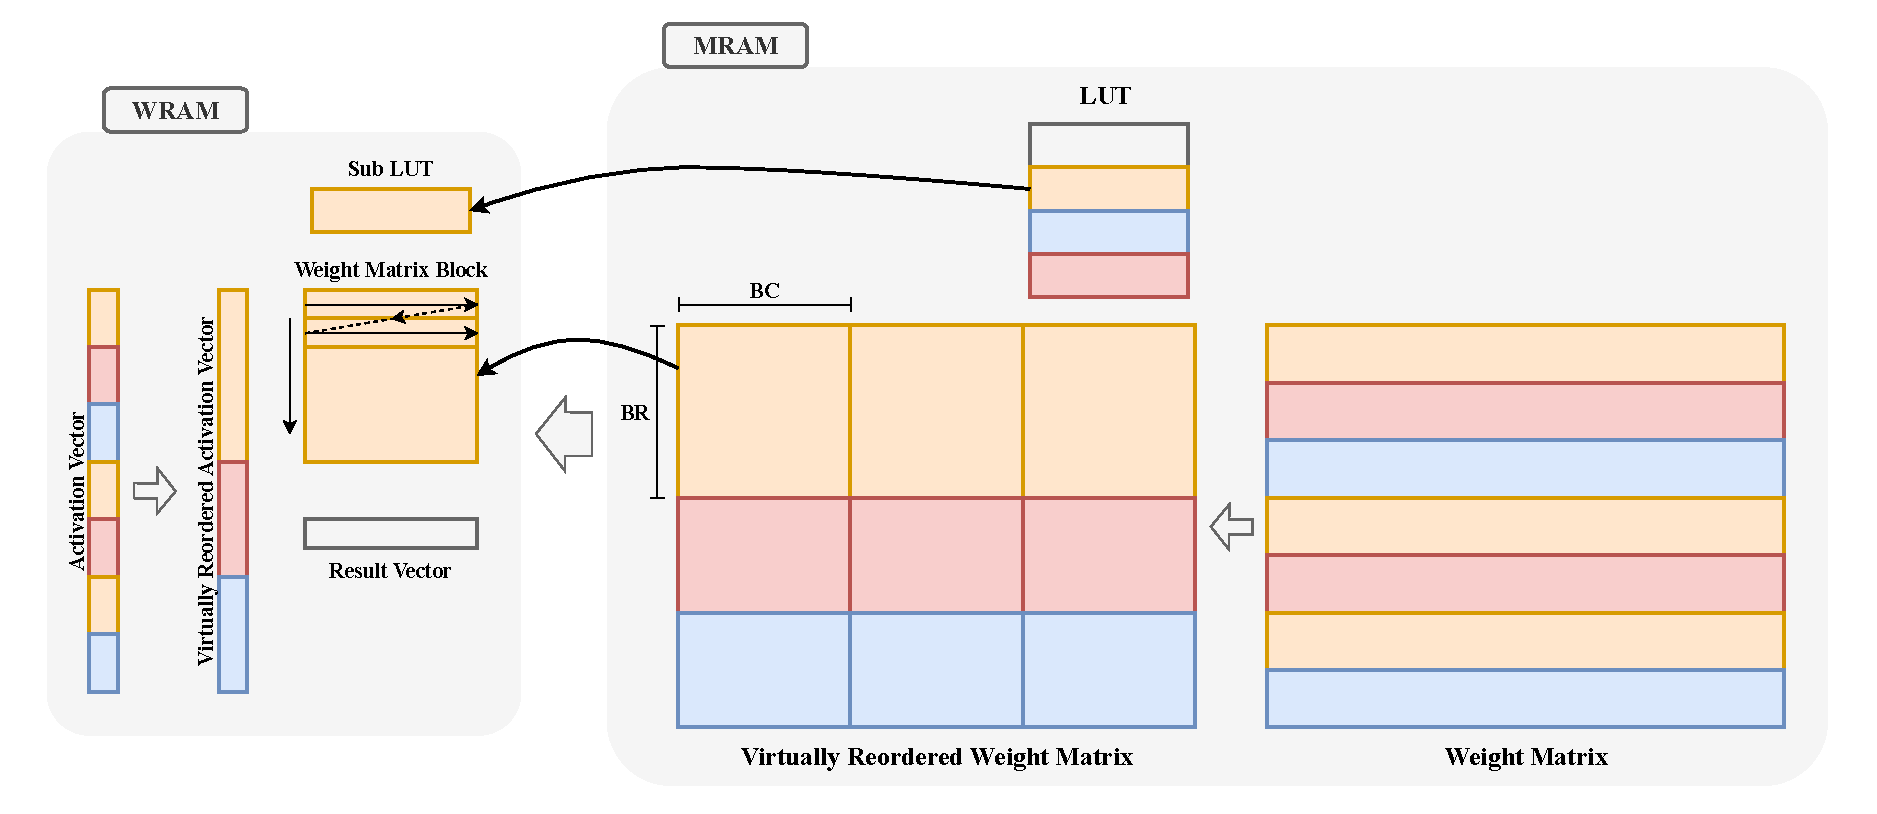
\includegraphics[width=0.9\textwidth]{figures/LUTRow.pdf}
	\caption{矩阵行重排优化计算示意图}
    \label{LUTRow}
\end{figure}

\begin{algorithm}[!ht]
    \caption{窄权重矩阵行重排的矩阵向量乘算法-LUTRow}
    \label{LUT_Row}
    \begin{algorithmic}[1]
        \Require $Vector[M], Matrix[M][N], LUT[256][256], FP8\_to\_INT32[256]$; % input
        \Ensure $Result\_8[N]$; % output

        \For{$i \gets 0$ \textbf{to} $15$}
            \State $\textbf{define}\; SubLUT[16][256]$
            \State $\textbf{mram\_read}(SubLUT, LUT[16i \cdots 16i + 15])$
            \Comment{\textcolor{blue}{parallel in 16 for each tasklet}}
            \For{$j \gets 0$ \textbf{to} $M - 1$}
                \If{$Vector[j] \;\textbf{not in}\; [16i, 16i+15]$}
                    \State \textbf{continue}
                \EndIf
                \State $\textbf{define}\; MatRow[N]$
                \State $\textbf{mram\_read}(MatRow, Matrix[j])$
                \Comment{\textcolor{blue}{parallel in N for each tasklet}}
                
                \For{$k \gets 0$ \textbf{to} $N-1$}
                \Comment{\textcolor{blue}{parallel in N for each tasklet}}
                    \State $Result[k] \gets Result[k] + SubLUT[Vector[j] \& \text{0xF}][MatRow[k]]$
                \EndFor
            \EndFor
        \EndFor

        % 调用二分查找函数
        \State $\textbf{define}\; Result\_32[N]$
        \State $Result\_8 \gets \textbf{BinarySearch}(Result\_32, FP8\_to\_INT32)$
        \Comment{\textcolor{blue}{parallel in N for each tasklet}}
        \State \Return $Result\_8$
    \end{algorithmic}
\end{algorithm}

此时没有任何新增的数据结构,WRAM的空间一定是放得下的,现在来计算WRAM的读写次数。在使用行重排之前,每次载入子查找表,每个tasklets需要完整地读一遍激活向量,4096次结果向量的读取和写入,得到WRAM的激活向量和结果向量的总次数为4096+128*4096/16+4096*2/16=36.5K read。而使用了行重排之后,假设刚好每次载入子查找表时,激活向量值域落在子查找表区间的行数都为256,那么每个tasklets只需要读写2次结果向量,但是对应子矩阵的激活向量需要重新读128次,则相应的总次数为4096+256+256x128/16+2=6K,有将近6倍的提升。

\subsection{宽矩阵列重排}
对于宽矩阵($128\times 4096$),我们可以观察到,当激活向量中的某个元素和权重矩阵的一行做乘积时,需要频繁地查找子查找表以获取乘积,然而由于矩阵权重为8bit,总共只有256种值,对应的乘积也只有256种值,因此理论上最多只需要查询256次LUT,但是现实的计算情况是矩阵一行中的每一个元素都重新去查询LUT,一共查询了4096次。如果将矩阵的一行按照数值排序,相同的连续数值只需要查表一次,这样就能避免重复查询LUT,提高访存效率。

按照此思想,我们提出列重排如图\ref{LUTRow:Construct}所示,为方便展示工作原理,这里以3bit数据位宽和一个16个元素的向量为例,对于权重矩阵的每一行,首先我们保留其索引值,按照元素值进行排序,排序后我们构建一个8个元素的桶(数组)对应3bit数据的所有取值情况,对权重矩阵每一行0-7数值出现的次数进行计数,计数完成后,对于着8个桶,我们称之为Delim数组,$Delim[i]$代表的含义就是值为i的元素出现的次数;接下来设置状态转移方程为\ref{DelimDP}。

\begin{equation}
    \text{delim}[i] = \begin{cases}
        \text{delim}[i] - 1, & i = 0 \\
        \text{delim}[i] + \text{delim}[i - 1], & i > 0
    \end{cases}
    \label{DelimDP}
\end{equation}

这样更新之后,Delim才被真正称之为分界数组,然后再将排序后的索引构成的Index数组替换为权重矩阵对应的行向量即可。这个时候delim数组的值就是指示着矩阵元素值发生变化的分界线。使用这样两个数据结构进行GEMV运算,如果确定了激活向量的元素的值V为2后,相当于确定了要查找的子查找表(哪一行),然后读取Delim数组可以知道,索引$(0,7]$的元素值都是1,因此可以通过查找LUT确定这个7个数的乘积都为1(uint8查找表),再读取载入的Index数组确定累加到结果向量的索引完成计算。

\begin{figure}[htbp!]
	\centering
	\subfigure[列重排Index和Delim数组构建]{
		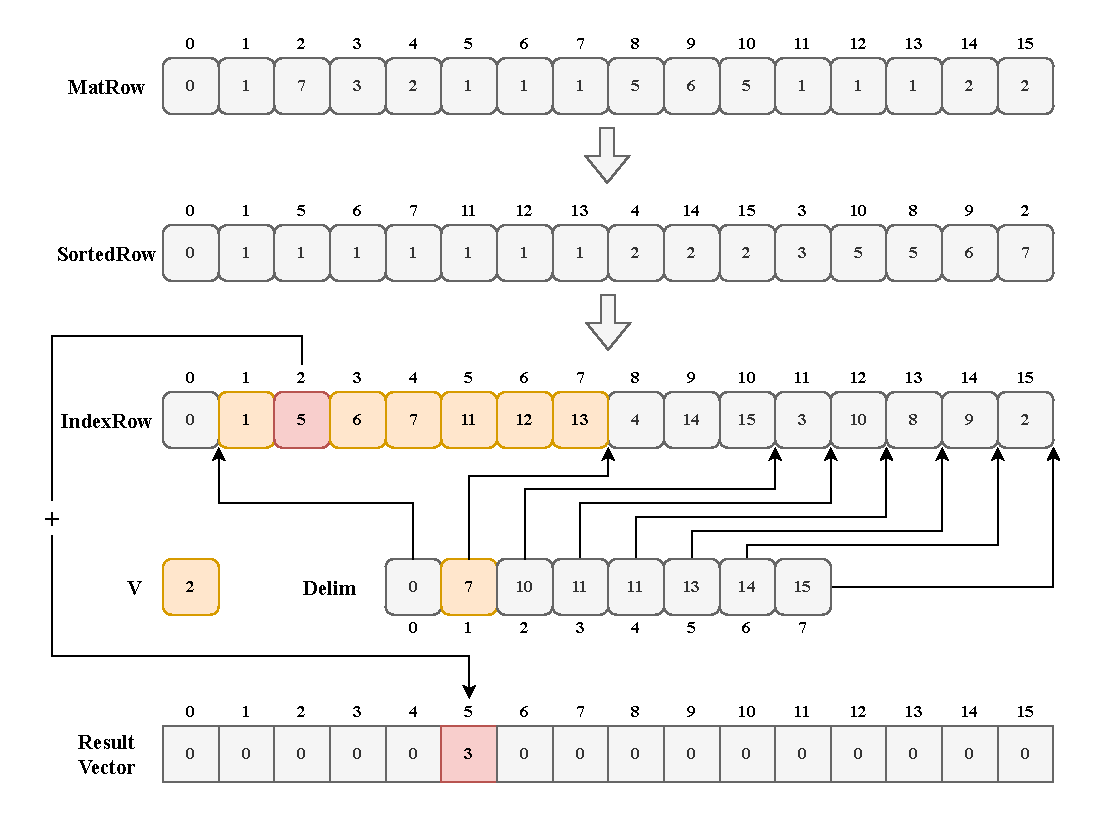
\includegraphics[width=0.5\textwidth]{figures/LUTCol.pdf}
		\label{LUTRow:Construct}}
	\subfigure[列重排并行计算优化]{
		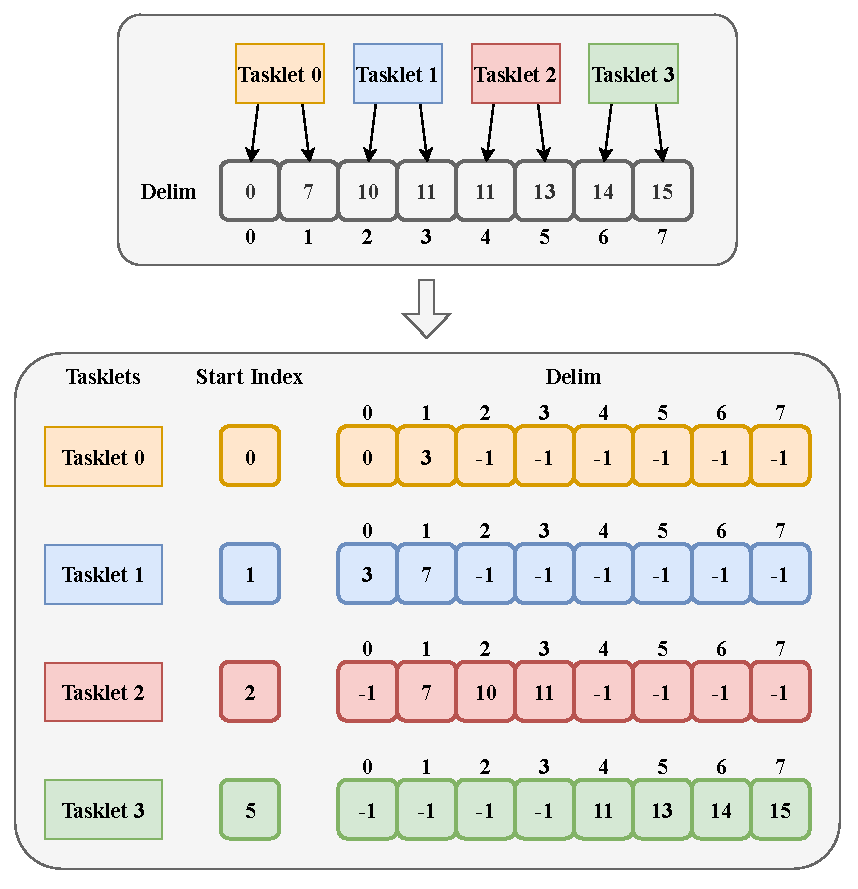
\includegraphics[width=0.4\textwidth]{figures/LUTColParallel.pdf}
        \label{LUTRow:Parallel}}
	\label{LUTRow}
	\caption{矩阵列重排优化计算示意图}
\end{figure}

但是由于数据的分布情况未知,简单按照Delim长度平均分配给个线程的任务可能出现严重的负载不均,无法充分利用DPU的并行计算能力。可以看到图\ref{LUTRow:Parallel}中,这16个元素的向量交由4个tasklet进行数据划分执行GEMV,如果按照简单地Delim数组长度平均分,即tasklet0负责Delim数组中索引0和1的计算,tasklet1负责2和3等等,那么就出现负载不均衡:tasklet0负责了8个元素的计算,几乎占据了整个向量计算量的一半,而其他tasklet的计算量非常低,甚至有些只有两个元素的计算量,这些tasklet计算完成后就会被闲置等待tasklet0完成工作。回到实际情况,试想一种极端情况:权重矩阵的某一行4096个元素,值全部都是1,这样所有的计算任务都会交由tasklet0执行,其他线程需要等待tasklet0计算完成才能进行下一行的计算,性能会大大降低。因此为了负载均匀,需要重新设计Delim数组的形式:为每个tasklet配备一个Delim数组,然后将任务均分到每个tasklet独享的Delim数组中。如图\ref{LUTRow:Parallel}所示,将前4个元素的计算分给tasklet0,则tasklet0需要执行一个值为0的计算和三个值为1的计算,那么只需要在Delim数组的0号索引填0,一号索引填3即可,在二号索引填-1表示任务结束不用继续读取Delim数组;tasklet1负责5-8号元素的计算,需要执行四个值为1的计算,只需要在一号索引填7,Start Index处填1表示任务起始的计算值,这样tasklet1就会从1号索引的前一号索引读取起始位置为3+1=4,然后读取4、5、6、7号元素执行计算。其他的tasklet类似。如此以来就能避免负载不均衡的问题。给出对应的算法表示\ref{LUT_Col}。

\begin{algorithm}[!ht]
    \caption{宽权重矩阵列重排的矩阵向量乘算法-LUTCol}
    \label{LUT_Col}
    \begin{algorithmic}[1]
        \Require $Vector[M], DelimMat[M][16][257], IndexMat[M][N], LUT[256][256], FP8\_to\_INT32[256]$; % input
        \Ensure $Result\_8[N]$; % output

        \State $\textbf{define}\; SubLUT[16][256]$
        \State $\textbf{define}\; IndexRow[N]$
        \State $\textbf{define}\; Delim[257]$

        \For{$i \gets 0$ \textbf{to} $15$}
            \State $\textbf{mram\_read}(SubLUT, LUT[16i \cdots 16i + 15])$
            \Comment{\textcolor{blue}{parallel in 16 for each tasklet}}
            \For{$j \gets 0$ \textbf{to} $M - 1$}
                \If{$Vector[j] \;\textbf{not in}\; [16i, 16i+15]$}
                    \State \textbf{continue}
                \EndIf
                
                \State $\textbf{mram\_read}(IndexRow, IndexMat[j])$
                \Comment{\textcolor{blue}{parallel in N for each tasklet}}
                \State $\textbf{mram\_read}(Delim, DelimMat[j][tasklet\_id])$

                \State $k \gets Delim[0]$
                \While{$Delim[k] \neq -1$}
                    \State $product \gets SubLUT[Vector[j] \& \text{0xF}][k]$
                    \For{$l \gets (\textbf{if } k=0 \textbf{ then } 0 \textbf{ else } Delim[k-1])$ \textbf{to} Delim[k]}
                        \State $Result[IndexRow[l]] \gets Result[IndexRow[l]] + product$
                    \EndFor
                    \State $k \gets k + 1$
                \EndWhile
            \EndFor
        \EndFor

        % 调用二分查找函数
        \State $\textbf{define}\; Result\_32[N]$
        \State $Result\_8 \gets \textbf{BinarySearch}(Result\_32, FP8\_to\_INT32)$
        \Comment{\textcolor{blue}{parallel in N for each tasklet}}
        \State \Return $Result\_8$
    \end{algorithmic}
\end{algorithm}

相比算法\ref{LUT_Block},MRAM中多了DelimMat,Matrix变为IndexMat,因为需要记录索引因此矩阵的元素从一字节变为两字节,MRAM仍然足够;WRAM中多了16个Delim数组,大概占用8KB的空间,且MatRow变为IndexRow多占用4KB空间,一共多占用12KB,如果此时宽矩阵的行数为128较小,激活向量占用不了4KB,总共占用WRAM空间53KB,剩余11KB给16个线程分配堆栈空间足够。同时每个tasklet在处理一行矩阵时由原来的4096次查表,变成了现如今最多256次查表,仅仅只是多读取了一个Delim数组,每行矩阵大概由原本的8K reads变为4.5K reads,差不多有两倍的性能提升。

\section{本章小结}
本章主要是介绍了在UPMEM硬件上对GEMV算子的软件优化,介绍了基本量化方式和查找表基础。在此基础上提出基于查找表分块的矩阵向量乘算法LUTBlock,该算法拥有非常号的WRAM数据局部性,充分优化了数据的流动。随后,针对Llama2-7B推理过程中MHSA涉及到常见的两种矩阵尺寸,分别是$4096\times 128$(窄矩阵)和$128\times 4096$(宽矩阵)分别做出了优化:行重排(LUTRow)和列重排(LUTCol),充分考虑GEMV计算中访问WRAM的特征,优化寄存器局部性,减少无意义的内存读写。